\documentclass[11pt]{article}
\usepackage{graphicx}

\begin{document}
	\begin{center}
		\begin{Large}
			Assignment No 7
		\end{Large}
	\end{center}•
	Aim:Implementation of code optimization techniques such as common sub-expression elemination.\\
	
	\noindent
	Objective:
	\begin{enumerate}
		\item To understand the code optimization phase..
		\item To learn how to eleminate common subexpressions from the given input ..
	\end{enumerate}•
	
	\noindent
	Software Requirement:
	\begin{enumerate}
		\item Linux Operating System
		\item GCC compiler
	\end{enumerate}•
	
	\noindent
	Consider a set S consisting of all the elements related to a program.The mathematical model is given as below, S={s,e,X,Y,Fme,DD,NDD,Mem shared} Where, s = Initial State\\ e = End State\\
	X	= Input data. Here it is Expression with 3 tokens or 5 tokens. Exampleof expressions: t1 = a * b or x = t1\\
	Y	= Output. Here output is printing a table that do not contains commonsub-expressions.\\
	Fme = Algorithm/Function used in program.for eg.{store(),searchleft(),searchright()}\\
	DD = Deterministic Data\\
	NDD = Non deterministic Data Mem shared = Memory shared by processor.\\
	
	\noindent
	THEORY :\\
	Code Optimization :\\
	Optimization is the process of transforming a piece of code to make more efficient (either in terms of time or space) without changing its output or side-effects. The only difference visible to the codes user should be that it runs faster and/or consumes less memory. It is really a misnomer that the name implies you are finding an ”optimal” solution in truth, optimization aims to improve, not perfect, the result.\\
	
	Many optimization problems are NP-complete and thus most optimization algorithms rely on heuristics and approximations. It may be possible to come up with a case where a particular algorithm fails to produce better code or perhaps even makes it worse. However, the algorithms tend to do rather well overall.\\
	
	\noindent
	When and Where To Optimize :\\
	The intermediate code, to streamline, rearrange, compress, etc. in an effort to reduce the size of the abstract syntax tree or shrink the number of TAC instructions. Others are applied as part of final code generationchoosing which instructions to emit, how to allocate registers and when/what to spill, and the like. And still other optimizations may occur after final code generation, attempting to re-work the assembly code itself into something more efficient.\\
	
	Optimization can be very complex and time-consuming; it often involves multiple subphases, some of which are applied more than once. Most compilers allow optimization to be turned off to speed up compilation (gcc even has specific flags to turn on and off individual optimizations.)\\
	
	\noindent
	Basic types of Optimizations: \\
	\begin{enumerate}
		\item  Local Optimization :\\Local Optimization focuses on:
		\begin{enumerate}
			\item Elimination of redundant operations
			\item Effective instruction scheduling
			\item Effective register allocation.
		\end{enumerate}•
		
		\item Optimization is considered local if it is done at a basic block level(a sequence of instruction where there is no branch in and out through its entirety).
		\begin{enumerate}
			\item Constant Folding :\\
			Constant folding refers to the evaluation at compile-time of expressions whose operands are known to be constant. In its simplest form, it involves determining that all of the operands in an expression are constant-valued, performing the evaluation of the expression at compile-time, and then replacing the expression by its value. If an expression such as 10 + 2 * 3 is encountered, the compiler can compute the result at compile-time (16) and emit code as if the input contained the result rather than the original expression. Similarly, constant conditions, such as a conditional branch if a ¡ b goto L1 else goto L2 where a and b are constant can be replaced by a Goto L1 or Goto L2 depending on the truth of the expression evaluated at compile-time.
			\item Constant Propagation :\\
			If a variable is assigned a constant value, then subsequent uses of that variable can be replaced by the constant as long as no intervening assignment has changed the value of the variable. Consider this section from our earlier Fibonacci example. On the left is the original, on the right is the improved version after constant propagation, which saves three instructions and removes the need for three temporary variables:\\
			tmp4 = 0 ;\\
			f0 = tmp4 ; tmp5 = 1 ;\\
			f1 = tmp5 ; tmp6 = 2 ;\\
			i = tmp6 ;\\
			f0 = 0 ; f1 = 1 ; i = 2 ;\\
			\item Copy Propagation :\\
			This optimization is similar to constant propagation, but generalized to non-constant values. If we have an assignment a = b in our instruction stream, we can replace later occurrences of a with b (assuming there are no changes to either variable in-between). Given the way we generate TAC code, this is a particularly valuable optimization since it is able to eliminate a large number of instructions that only serve to copy values from one variable to another.
			\item Dead Code Elimination :\\
			If an instructions result is never used, the instruction is considered ”dead” and can be removed from the instruction stream. So if we have\\
			tmp1 = tmp2 + tmp3 ;\\
			and tmp1 is never used again, we can eliminate this instruction altogether. However, we have to be a little careful about making assumptions, for example, if tmp1 holds the result of a function call:\\
			tmp1 = LCall Binky;\\
			Even if tmp1 is never used again, we cannot eliminate the instruction because we cant be sure that called function has no side-effects. Dead code can occur in the original source program but is more likely to have resulted from some of the optimization techniques run previously.
			\item Common Subexpression Elimination :\\
			Two operations are common if they produce the same result. In such a case, it is likely more efficient to compute the result once and reference it the second time rather than re-evaluate it. An expression is alive if the operands used to compute the expression have not been changed. An expression that is no longer alive is dead.
			
		\end{enumerate}•
	\end{enumerate}•
	
	\noindent
	Consider following example:\\
	tmp1 = 1 + 20 ;\\ tmp2 = -x ;\\ x = tmp1 * tmp2 ;\\ tmp3 = x * x ;\\ tmp4 = x / y ;\\ y = tmp3 + tmp4 ;\\ tmp5 = x / y ;\\ tmp6 = x * x ;\\ z = tmp5 / tmp6 ;\\ y = z ;\\
	What subexpressions can be eliminated? How can valid common subexpressions (live ones) be determined? Here is an optimized version, after constant folding and propagation and elimination of common sub-expressions:\\
	tmp2 = -x ;\\ x = 21 * tmp2 ; \\tmp3 = x * x ;\\ tmp4 = x / y ;\\ y = tmp3 + tmp4 ;\\ tmp5 = x / y ;\\ z = tmp5 / tmp3 ;\\ y = z ;\\
	\begin{enumerate}
		\item Global Optimization :\\
		Global Optimization focuses on:\\
		\begin{enumerate}
			\item Same techniques performed by local optimization but at multibasic-block level
			\item Code modifications to improve the performance of loops.
		\end{enumerate}•
		
		\item Both local and global optimization use a control flow graph to represent the program, and a data flow analysis algorithm to trace the flow of information.
		\item Peephole Optimizations :
		\begin{enumerate}
			\item Peephole Optimization works by sliding a several-instruction window (a peephole) over the target code, and looking for suboptimal patterns of instructions.
			\item The patterns to look for are heuristic, and typically based on special instructions available on a given machine.
			\item The peephole is a small, moving window on the target program. The code in the peephole need not contiguous, although some implementations do require this.it is characteristic of peephole optimization that each improvement may spawn opportunities for additional improvements.
			\item Peephole optimization is a pass that operates on the target assembly and only considers a few instructions at a time (through a ”peephole”) and attempts to do simple, machinedependent code improvements.
			\item For example, peephole optimizations might include elimination of multiplication by 1, elimination of load of a value into a register when the previous instruction stored that value from the register to a memory location, or replacing a sequence of instructions by a single instruction with the same effect.
			\item We shall give the following examples of program transformations that are characteristic of peephole optimizations:
			\begin{enumerate}
				\item 	Redundant-instructions elimination
				\item Flow-of-control optimizations
				\item Algebraic simplifications
				\item Use of machine idioms
				\item Unreachable Code
				
			\end{enumerate}•
			
		\end{enumerate}•
		
		\item Loop Optimization :
		\begin{enumerate}
			\item Loop optimization is the process of the increasing execution apeed and reducing the overheads associated of loops.
			\item It plays an important role in improving cache performance and making effective use of parallel processing capabilities.
			\item Most execution time of a scientific program is spent on loops; as such, many compiler optimization techniques have been developed to make them faster.
			\item common loop transformations:
			\begin{enumerate}
				\item Code Fission:\\
				loop fission attempts to break a loop into multiple loops over the same index range but each taking only a part of the lopp’s body.
				\item Code Fusion:\\
				When two adjacent loops would iterate the same number of times,their bodies can be combined as long as they make no reference to each others data.
				\item Spitting/peeling:\\
				Loop spliting attempts to simplify a loop or eliminate dependencies by breaking it into multiple loops which have the same bodies but iterate over different contiguous portions of the index range.A useful special case is loop peeling,which can simplify a loop with a problematic first iteration by performingthat iteration seperately before entering the loop.
				\item Code Motion:\\
				Code motion (also called code hoisting) unifies sequences of code common to one or more basic blocks to reduce code size and potentially avoid expensive re-evaluation. The most common form of code motion is loop-invariant code motion that moves statements that evaluate to the same value every iteration of the loop to somewhere outside the loop.
				
			\end{enumerate}•
			
		\end{enumerate}•
		
	\end{enumerate}•
	
	\noindent
	Command :\\
	\$ gcc $<program name>$.c\\ \$ ./a.out\\
	
	\noindent
	CONCLUSION :\\	
	Thus, we have implemented code optimization technique by eliminating common sub expression.
	
	\begin{center}
		\begin{tabular}{|c|c|c|c|c|}
			•$Roll$ $No$ & $Name$ $of$ $Student$ & $Date$ $of$ $performance$ & $Date$ $of$ $Checking$ & $Signature$ $of$ $Staff$ \\ \hline
			$BECOC357$ & Sunny Shah&29 / 09 / 2017& 06 / 10 / 2017  & \\ \hline
		\end{tabular}•
	\end{center}•
	\newpage
	\section{PLAGARISM REPORT :}
	\begin{figure}[h!]
		\centering
		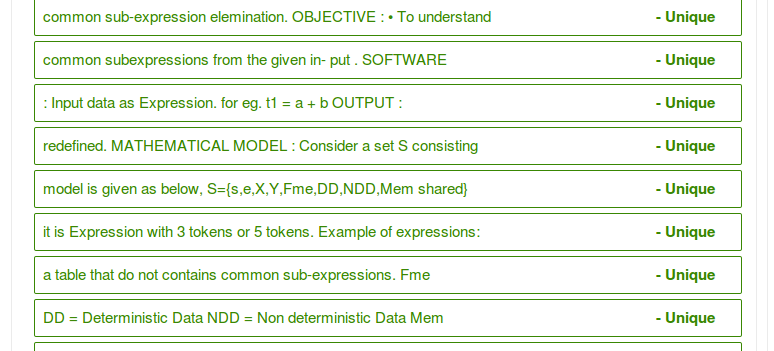
\includegraphics[height=5in,width=6in]{plagiarism7.png}
		\caption{Plagarism Checker www.smallseotools.com/plagarism-checker}
	\end{figure}
	\newpage
\end{document}

